% This is "sig-alternate.tex" V2.0 May 2012
% This file should be compiled with V2.5 of "sig-alternate.cls" May 2012
%
% This example file demonstrates the use of the 'sig-alternate.cls'
% V2.5 LaTeX2e document class file. It is for those submitting
% articles to ACM Conference Proceedings WHO DO NOT WISH TO
% STRICTLY ADHERE TO THE SIGS (PUBS-BOARD-ENDORSED) STYLE.
% The 'sig-alternate.cls' file will produce a similar-looking,
% albeit, 'tighter' paper resulting in, invariably, fewer pages.
%
% ----------------------------------------------------------------------------------------------------------------




%%%%%% TO   DOO
% Intro - GraphCHI GraphLab? Related work, defend distributed approach
% Methodologies: pseudocode, heuristics

% PARMETIS !!!!
% Build table of weak/strong scaling time plots
% Build table of quality plots


%Robert:
% Motivating Applications
% Related Work


\documentclass{sig-alternate}


\usepackage{xspace}
\usepackage{url}
\usepackage{color}
\usepackage{algorithm2e}
\usepackage{amsmath}

\usepackage[table]{xcolor}
\usepackage{booktabs}

% Pienta's defines:
\DeclareMathOperator*{\argmax}{\arg\!\max}

\newcommand{\todo}[1]{\textcolor{red}{[#1]}}
\newcommand{\robert}[1]{\textcolor{OliveGreen}{[#1 -R]}}
\newcommand{\acar}[1]{\textcolor{blue}{[#1 -A]}}
\newcommand{\polo}[1]{\textcolor{red}{[#1 -P]}}
\newcommand{\alex}[1]{\textcolor{Mahogany}{[#1 - A]}}

\newcommand{\xourname}{Grasp}
\newcommand{\name}{\textsc{\xourname}\xspace}
\newcommand{\ourmethod}{\name}
\newcommand{\ourmethodtitle}{Grasp\xspace}

\newcommand{\expparm}{$t_\alpha$\xspace}
\newcommand{\numrestreamsparm}{n_s}
\newcommand{\numprocsparm}{$p$\xspace}


\newcommand{\largestgraphedges}{10000\xspace}
\newcommand{\largestgraphtime}{100 seconds}

\newcommand{\ignore}[1]{}


\begin{document}
%
% --- Author Metadata here ---
\conferenceinfo{KDD}{'15 Sydney, Australia}
%\CopyrightYear{2007} % Allows default copyright year (20XX) to be over-ridden - IF NEED BE.
%\crdata{0-12345-67-8/90/01}  % Allows default copyright data (0-89791-88-6/97/05) to be over-ridden - IF NEED BE.
% --- End of Author Metadata ---

\title{GraSP: Distributed Streaming Graph Partitioning}
%\subtitle{[Extended Abstract]
%\titlenote{A full version of this paper is available as
%\textit{Author's Guide to Preparing ACM SIG Proceedings Using
%\LaTeX$2_\epsilon$\ and BibTeX} at
%\texttt{www.acm.org/eaddress.htm}}}
%
% You need the command \numberofauthors to handle the 'placement
% and alignment' of the authors beneath the title.
%
% For aesthetic reasons, we recommend 'three authors at a time'
% i.e. three 'name/affiliation blocks' be placed beneath the title.
%
% NOTE: You are NOT restricted in how many 'rows' of
% "name/affiliations" may appear. We just ask that you restrict
% the number of 'columns' to three.
%
% Because of the available 'opening page real-estate'
% we ask you to refrain from putting more than six authors
% (two rows with three columns) beneath the article title.
% More than six makes the first-page appear very cluttered indeed.
%
% Use the \alignauthor commands to handle the names
% and affiliations for an 'aesthetic maximum' of six authors.
% Add names, affiliations, addresses for
% the seventh etc. author(s) as the argument for the
% \additionalauthors command.
% These 'additional authors' will be output/set for you
% without further effort on your part as the last section in
% the body of your article BEFORE References or any Appendices.

\numberofauthors{3} %  in this sample file, there are a *total*
% of EIGHT authors. SIX appear on the 'first-page' (for formatting
% reasons) and the remaining two appear in the \additionalauthors section.
%
\author{
% You can go ahead and credit any number of authors here,
% e.g. one 'row of three' or two rows (consisting of one row of three
% and a second row of one, two or three).
%
% The command \alignauthor (no curly braces needed) should
% precede each author name, affiliation/snail-mail address and
% e-mail address. Additionally, tag each line of
% affiliation/address with \affaddr, and tag the
% e-mail address with \email.
%
% 1st. author
\alignauthor Casey Battaglino\\
       \affaddr{Georgia Institute of Technology}\\
       \email{cjbattagl@gatech.edu}
% 2nd. author
\alignauthor Robert Pienta\\
       \affaddr{Georgia Institute of Technology}\\
       \email{pientars@gatech.edu}
% \alignauthor Guy Fieri\\
\alignauthor Richard Vuduc\\
       \affaddr{Georgia Institute of Technology}\\
       \email{richie@cc.gatech.edu}
%
}
% There's nothing stopping you putting the seventh, eighth, etc.
% author on the opening page (as the 'third row') but we ask,
% for aesthetic reasons that you place these 'additional authors'
% in the \additional authors block, viz.
%\additionalauthors{Additional authors: John Smith (The Th{\o}rv{\"a}ld Group,
%email: {\texttt{jsmith@affiliation.org}}) and Julius P.~Kumquat
%(The Kumquat Consortium, email: {\texttt{jpkumquat@consortium.net}}).}
%\date{30 July 1999}
% Just remember to make sure that the TOTAL number of authors
% is the number that will appear on the first page PLUS the
% number that will appear in the \additionalauthors section.

\maketitle
%!TEX root=kdd15_workshop_main.tex
\begin{abstract}
The size of real-world graph data sets continues to grow past the limits of commodity machines. In distributing large-scale graph mining approaches, a first step is often partitioning the data across machines in a way that reduces communication volume while simultaneously promoting load-balance. 
While graph partitioning is a mature field, recent work has shown that low-overhead streaming heuristics can perform competitively with heavyweight, offline graph partitioners for many real-world graphs. 

In this work we investigate the process of partitioning a social graph using a \emph{distributed, streaming} partitioner, \ourmethod, which makes partition decisions as each vertex is read from memory, simulating an online algorithm that must process nodes as they arrive. 
We make use of the MPI paradigm, ubiquitous in the HPC world, to promote \ourmethod as a simple library to substitute for existing libraries such as parMetis. 

\ourmethod is the first MPI implementation of streaming partitioning that we are aware of, and demonstrates performance far exceeding existing partitioners while providing comparable results. We demonstrate the scalability of \ourmethod on up to 1024 compute nodes of NERSC's Edison supercomputer.
\end{abstract}



% A category with the (minimum) three required fields
\category{H.4}{Information Systems Applications}{Miscellaneous}
%A category including the fourth, optional field follows...
\category{D.2.8}{Software Engineering}{Metrics}[complexity measures, performance measures]
\terms{Theory}

\keywords{graph partitioning, streaming graph partitioning}

%!TEX root=kdd15_workshop_main.tex
\section{Introduction}

% main point
We consider the problem of partitioning a streaming graph on a distributed memory system.
We are particularly interested in doing so for the kinds of irregular graphs that arise in applications like fraud detection, bioinformatics, and social and information network analysis, among numerous others.
%
%\subsection{Graph Partitioning}
%motivation: this is fluff; remove
\ignore{
From fraud detection to bioinformatics, large-scale graph mining and analytics provide access and deeper insight into the rich patterns in our data.
The availability and granularity of our network data is growing at an impressive pace.
With billions of online interactions, social networks (like e-commerce or the Twittersphere) have grown so immense and rich with data that they cannot easily be analyzed on a single machine.
Spreading these large graphs across multiple systems for analysis often takes complex algorithms with long computation times.
Modern data analytics moves fast, and the partitioning of massive graphs should too.
}
%
%Distributed, irregular algorithms such as large-scale graph mining often encounter bottlenecks in network communication and load imbalance~\cite{challenglums}.
The speed of mining algorithms on such graphs, at scale, is often limited by bottlenecks in network communication and load imbalance~\cite{challenglums}.
Partitioning is the common preprocessing step to find a mapping of the data to processors of the system that alleviates these two issues;
%Graph partitioning is the general problem of dividing a graph into separate components with desired properties;
in distributed computing the desired objective is generally the minimization of inter-partition edges (to minimize communication) subject to balanced partition size (to favor load balance).

Formally, we wish to partition the nodes of a graph into $k$ balanced components with capacity $(1+\epsilon)\frac{N}{k}$, such that the number of edges crossing partition boundaries is minimized. Partitioning with these two requirements can be reduced to the minimum-bisection problem~\cite{Garey:1979:CIG:578533} and is therefore NP-Complete. 
Thus, computing an optimal mapping is generally computationally infeasible, and heuristic approaches are taken. 

\begin{figure}[ht]
\centering
  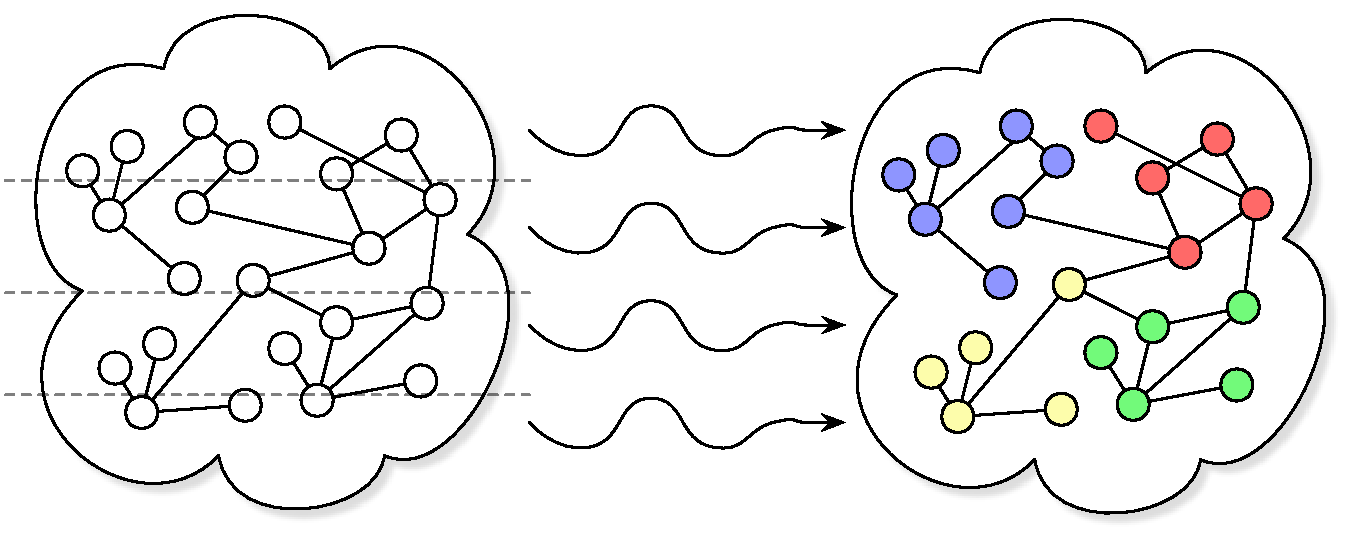
\includegraphics[width=0.7\columnwidth]{figures/coverfig.pdf}
  %\caption{Partition speed of various Kronecker graphs.}
  \label{fig:coverfig}
  \caption{Parallel streaming partitioning.}
\end{figure}

To illustrate the role of partitioning on performance, consider a parallel Breadth-First Search (BFS) where a graph's vertices are partitioned between two machines in a `1D' distribution~\cite{Buluc2D}. During each BFS step, each process must communicate all newly explored target vertices to process that owns them. In Figure~\ref{fig:0}, if we have 4 processes, all 14 nonzeros in the non-diagonal blocks must be communicated at some point. A good partitioner concentrates nonzeros in the diagonal blocks, thereby reducing communication.\footnote{Computing exact communication volume requires a hypergraph partitioner~\cite{hypergraph}.} 
>>>>>>> origin/rv

% \todo{In the figure: Differentiate the cut-edges and their associated non-zeroes from the internal edges, to emphasize that they are undersirable.}
\begin{figure}[h]
\centering
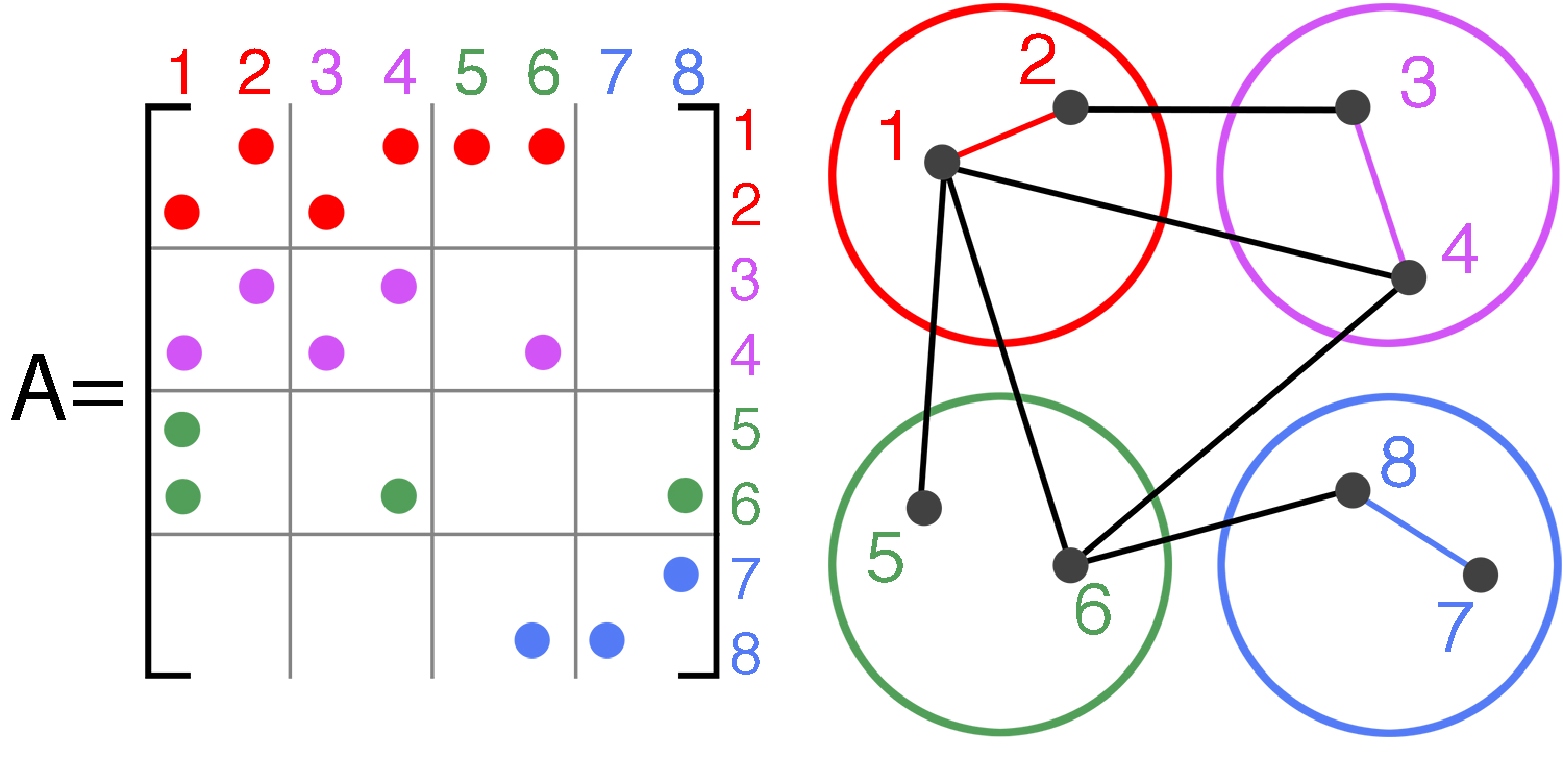
\includegraphics[width=0.85\columnwidth] {figures/graphpart1.pdf}
\caption[Caption for]{Graph 4-partition shown with corresponding adjacency matrix}
\label{fig:0}
\end{figure}

Offline graph partitioning algorithms have existed for dec\-ades. They work by storing the graph in memory with complete information about the edges. Many variants of these algorithms exist~\cite{gpsurvey} and range from spatial methods~\cite{Gilbert95geometricmesh} to spectral methods~\cite{arora2009expander}. Some of the most effective offline graph partitioners are multi-level partitioners, which recursively contract the graph to a small number of vertices, and then heuristically optimize the partitioning while expanding back to the original graph~\cite{karypis1998multilevel}.
These methods are especially effective on geometric graphs, that is, graphs that arise from some physical geometry, like the discretized finite element mesh of a physical object.
Parallel multi-level partitioners will serve as the baseline comparison for our implementation. 

\paragraph{Streaming Partitioning}
Streaming partitioning is the process of partitioning a graph in a single sweep, reading vertices and edges only once. Thus we incur $O(|V| + |E|)$ memory access, storage, and run time, with minimal overhead. Offline graph partitioners require the whole graph to be represented in memory, whereas streaming graph partitioning can process vertices as they arrive. This fits a model where input data arrive sequentially from a generating source (such as a web-crawler).

Partitioning a \SI{26}{\giga\byte} Twitter graph has been shown to take \SI[abbreviations=false]{8}{\hours} using the fastest offline algorithms, and only \SI{40}{\minutes} with the FENNEL streaming partitioner, with similar partition quality~\cite{tsourakakis2012fennel}. This also suggests that we could do multiple, iterative passes of a streaming partitioner, all in a fraction of the time that an offline partitioner would take to terminate. This technique and its convergence properties have been explored by Nishimura and Ugander~\cite{nishimura2013restream}. In this paper we demonstrate empirically that distributing this streaming partitioning process can reduce the run-time for problem of this magnitude to a matter of \emph{seconds}. 

\paragraph{Contributions}
We have developed \ourmethod, a fast, iterative, distributed streaming graph partitioner.
It works by restreaming the distributed graph with tempered partition parameters to achieve a fast, parallel \textit{k}-partitioning.
We make the following contributions:
\begin{itemize}
\item A \textbf{scalable} distributed, open-source partitioner implementation using MPI.
\item Support for \textbf{streaming} and restreaming partitioning regardless of stream order.
\item A robust method for automatically tuning \ourmethod parameters 
\end{itemize}




%!TEX root=kdd15_workshop_main.tex
\section{Methodology}
While there are many possible heuristics for streaming partitioning~\cite{Stanton:2012:SGP:2339530.2339722}, the most effective by far have been \emph{weighted, greedy} approaches. We keep track of the partition assignments of vertices streamed so far ($P_i^t$ for each process $i$ at time $t$). As each vertex $v$ is streamed, we count the edges from that vertex to each partition $|P_i^t \cap N(v)|$. This intuitively maximizes \emph{modularity}, the ratio of intra-partition edges to inter-partition edges. However, using this value on its own would result in all vertices being assigned to a single, large partition. Thus, we exponentially \emph{weight} the edge counts by the size of partitions $|P_i^t|$, relatively dampening the scores for partitions that are too large (but penalizing only lightly for small differences in size). This gives us two parameters: the linear importance of partition size to the score, $\alpha$, and the exponential rate at which increasing partition size incurs a greater penalty, $\gamma$. This yields the basic `FENNEL' algorithm~\cite{tsourakakis2012fennel}:

\begin{algorithm}
 Set all $P_i$ to $\emptyset$\;
 \ForEach{$v \in V(G)$ as it arrives at time $t$}{
   $j \gets \displaystyle \argmax_{i\in\{1,\dots,p\}}|P_i^t \cap N(u)| - \alpha \frac{\gamma}{2}|P_i^t|^{\gamma-1}$\;
   Add $v$ to set $P_j^{t+1}$\;
 }
 \caption{Serial streaming FENNEL partitioner}
\end{algorithm}

Exact computation of this algorithm as described is not possible in parallel, because $P_i^{t-1}$ must be known to compute $P_i^t$. A multi-threaded approximation of this algorithm is easily performed by relaxing this requirement and using $P_i^{t-p}$ to compute $P_i^t$, where $p$ is the number of threads. This resulted in only a small drop in partition quality in our experiments.

To compute this algorithm in distributed memory, a naive approach is to constantly broadcast partition assignments as they are computed. Unless we use synchronization (which involves a massive performance hit), this results in a drastic drop in partition quality because the latency across a network is high enough that partition assignments are perpetually out of date. 

Our implementation follows the methodology of `restreaming' partitioning'~\cite{nishimura2013restream}, which shows the single-pass algorithms of FENNEL and WDG~\cite{tsourakakis2012fennel,Stanton:2012:SGP:2339530.2339722} can be repeated over the same data in the same order, yielding a convergent improvement in quality. This approach has other benefits that we utilize:

\begin{itemize}
\item Partition data is only communicated between streams, yielding high parallelism.
\item Parameters ($\alpha, \gamma)$ can be `tempered' to achieve higher-quality, balanced results that avoid immediate global minima.
\end{itemize}

\subsection{\ourmethod}
\ourmethod operates on a distributed graph $G$ in distributed CSR format. We take as input the parameters $\alpha, \gamma$, the number of partitions \numprocsparm (assumed to be equal to the number of MPI processes), the number of re-streams $\numrestreamsparm$, and the `tempering' parameter \expparm. \ourmethod then performs $\numrestreamsparm$ iterative passes over the graph (in identical random order), multiplicatively increasing the balance parameter by \expparm with each pass. This promotes a high-quality but less-balanced partition early on, while further promoting balance with subsequent pass~\cite{nishimura2013restream}. 

In between each pass, the partition information is communicated across all processors using the MPI \textsc{AllGather} primitive, which is often optimized for a given network architecture. The pseudocode for \ourmethod is shown in Algorithm~\ref{alg:grasp}.


\begin{algorithm}
\ForPar{each process $p$}{
	$vorder \gets rand\_perm(\{0,\dots,|V(G_{local})|\})$\;
	Randomly assign local vertices to partitions $P_{i,p}^0$\;
}
\For{$run \gets \{ 1 \dots \numrestreamsparm \}$} {
	\ForPar{each process $p$}{
		\ForEach{$v \in vorder$}{
			$j \gets part(v)$\;
			$k \gets \displaystyle \argmax_{i\in\{1,\dots,p\}}|P_{i,p}^t \cap N(u)| - \alpha \frac{\gamma}{2}|P_{i,p}^t|^{\gamma-1}$\;
			Remove $v$ from set $P_{j,p}^{t}$\;
			Add $v$ to set $P_{k,p}^{t+1}$\;
		}
	}
	\textsc{MPI\_AllGather} global partition assignments\;
}
 \caption{Parallel Restreaming performed by \ourmethod.}
 \label{alg:grasp}
\end{algorithm}

This method is illustrated graphically in Fig.~\ref{fig:restream}.

\begin{figure}[ht]
\centering
  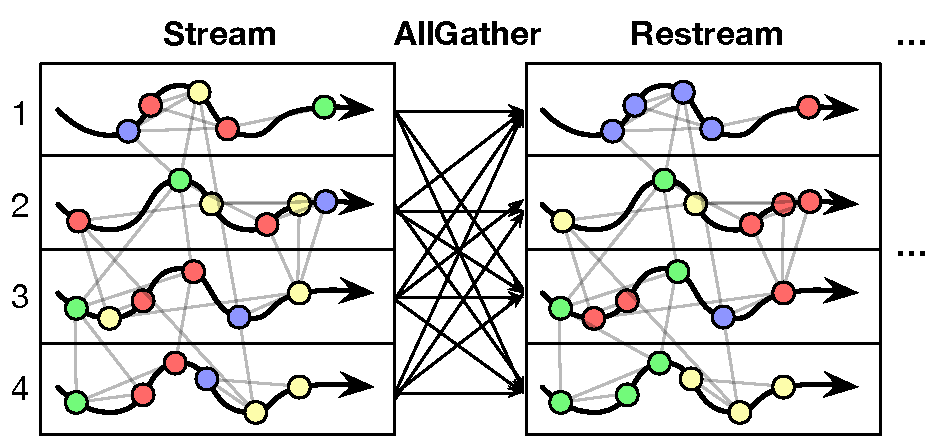
\includegraphics[width=1.0\columnwidth]{figures/restreamdiagram.pdf}
  %\caption{Partition speed of various Kronecker graphs.}
  \label{fig:restream}
  \caption{Two parallel restreaming steps on four processes.}
\end{figure}

Each process computes $O(\numrestreamsparm \cdot \frac{|E|+|V|}{p})$ work, and the network incurs a time of $\numrestreamsparm \cdot T_{allgather}(|V(G)|)$. 

%!TEX root=kdd15_workshop_main.tex
\section{Evaluation}

We ran our distributed experiments on the Edison machine at NERSC, featuring 5576 compute nodes with two 12-core Intel ``Ivy Bridge'' processors per node, and a Cray Aries interconnect. For scalability experiments we generated undirected Kronecker graphs of varying scale in parallel using the Graph500 Reference implementation~\cite{graph500}. 

We also measured the overall quality of partitions by the \textit{fraction of cut edges} $\lambda$.
\begin{align}\lambda = \frac{\text{Number of edges cut by partition}}{\text{Total number of edges}}\end{align}
The fraction of edges cut demonstrates the quality of the edge minimization aspect of partitioning the graph.

As a baseline, we can compare this to the expected quality of a random $k-$partition:
\begin{align}\lambda_r = \frac{k^2 - k}{k^2} = \frac{k-1}{k} \end{align}

Any partitioner that produces partitions with $\lambda < \lambda_r$ has improved the parallel locality of the partitions. 
We present $\lambda_{r,k}$ along with our one-pass, real network results in Table \ref{table:big}.

\subsection{Test Graphs}
We tested \ourmethod on both real and synthetic networks.
Real networks demonstrate \ourmethod's potential for use on real domain problems.
We also utilized synthetic graphs, because they allow better experimental control over size and structure.
\subsubsection{Real-world Graphs}
The SNAP dataset is a collection of real-world networks collected by Leskovec and collaborators~\cite{Leskovec-data, snapnets}. 
Many networks in the collection are power-law and scale-free representatives of social networks (such as collaboration networks, citation networks, email networks, and web graphs). We consider these to be ideal targets for streaming partitioning, because these domains are producing the vast majority of the `big-data' that is difficult to partition using traditional methods.

% We also speculate (but have no proof) that the `random' structure of scale-free networks better suits the random quality of streaming graph partitioning, whereas a spatially-oriented graph would be poorly suited (for instance, in a grid, a streaming partitioner would create many local pockets for one particular partition, whereas a spatial partitioner would recognize that the graph could be geometrically bisected).

\subsubsection{Synthetic Graphs}
To generate the test graphs we used the Graph500 Kronecker-Graph generator.
Kronecker graphs are commonly used in HPC graph benchmarks and testing and can be scaled arbitrarily large for testing purposes. 



\subsection{Quality}
In Table~\ref{table:big} we show some properties of our real test-graphs, as well as the performance of our streaming partitioner on them, for $k=2$ and $k=8$.
% As a note, the ratio of change in $\lambda$ from $k=2$ to $k=8$ was for the vast majority of cases within 1.5 and 2.2. 
% This suggests good scalability.


\begin{figure}
\caption{Basic properties of graphs in SNAP data set~\cite{Leskovec-data}, and $\lambda$ for one pass. $\lambda_{r,2}=0.5,\lambda_{r,8}=0.87$}
\rowcolors{2}{blue!05}{blue!15}
\centering
\small
{ \begin{tabular}{ *5r }    \toprule
\label{table:big}
\emph{Data Set} & $N$ & $nnz$  & $\lambda_{k=2}$ & $\lambda_{k=8}$ \\\midrule
soc-LiveJournal & 4,847,571 & 68,993,773  &0.234& 0.463\\
as-Skitter & 1,696,415 & 22,190,596  & 0.166&0.324\\
cit-Patents & 3,774,768 & 16,518,948  & 0.402&0.726\\
roadNet-CA & 1,971,281 & 5,533,214  & 0.186&0.360\\
web-Google & 916,428 & 5,105,039  &0.189&0.336\\
wiki-Talk & 2,394,385 & 5,021,410 &0.411&0.752\\
amazon0302 & 262,111 & 1,234,877 & 0.202&0.370\\
soc-Slashdot0902 & 82,168 & 948,464  &0.236&0.382\\
ca-AstroPh & 18,772 & 396,160 & 0.232&0.413\\
cit-HepPh & 34,546 & 421,578 & 0.343&0.646\\
email-EuAll & 265,214 & 420,045 & 0.280&0.538\\
Oregon-1 & 11,492 & 46,818  & 0.224&0.406\\
p2p-Gnutella04 & 10,879 & 39,994  & 0.415&0.747\\


 \hline
\end{tabular}\par
}
\end{figure}


%\begin{figure}
%\caption{Basic properties of graphs in SNAP data set~\cite{Leskovec-data}, and $\lambda$ for one pass. $\lambda_{r,2}=0.5,\lambda_{r,8}=0.87$}
%\rowcolors{2}{blue!05}{blue!15}
%\centering
%{ \begin{tabular}{ *5r }    \toprule
%\label{table:big}
%\emph{Data Set} & $N$ & $nnz$  & $\lambda, k=2$ & $\lambda, k=8$ \\\midrule
%amazon0302 & 262111 & 1234877 & 0.202&0.370\\
%as-Skitter & 1696415 & 22190596  & 0.166&0.324\\
%ca-AstroPh & 18772 & 396160 & 0.232&0.413\\
%cit-HepPh & 34546 & 421578 & 0.343&0.646\\
%cit-Patents & 3774768 & 16518948  & 0.402&0.726\\
%email-EuAll & 265214 & 420045 & 0.280&0.538\\
%Oregon-1 & 11492 & 46818  & 0.224&0.406\\
%p2p-Gnutella04 & 10879 & 39994  & 0.415&0.747\\
%roadNet-CA & 1971281 & 5533214  & 0.186&0.360\\
%soc-LiveJournal & 4847571 & 68993773  &0.234& 0.463\\
%soc-Slashdot0902 & 82168 & 948464  &0.236&0.382\\
%web-Google & 916428 & 5105039  &0.189&0.336\\
%wiki-Talk & 2394385 & 5021410 &0.411&0.752\\
% \hline
%\end{tabular}\par
%}
%\end{figure}


% We also note Figure~\ref{fig:4}, which illustrates the result of the streaming algorithm on a more spacial network (roadNet-CA). The `local' nonzeros are those points in the 8 diagonal blocks, while the `remote' edges are those outside. While a good partitioner would concentrate the vast majority of elements along the diagonal (which is possible because the graph has very high diameter), the streaming partitioner fails to recognize this quality, and each partition has vertices distributed somewhat randomly through the network. Nonetheless, the partition is decent (only 18 percent of edges are cut).

% \begin{figure}[h!]
% \centering
% 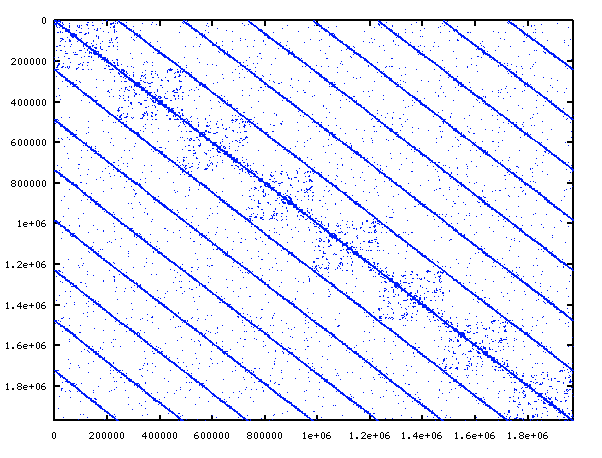
\includegraphics[width=0.8\columnwidth] {figures/roadNet-CA8.png}
% \caption[Caption for]{Spy plot of roadNet-CA 8-partition ($\lambda=0.177$). This illustrates how a streaming algorithm cannot take into account the spatial/planar properties of a graph.}
% \label{fig:4}
% \end{figure}


% In Figure~\ref{fig:kronspeed} however, we increase the $p$-value on a single ER graph. We see that the partition quality significantly decreases. 
% This is to be expected of all partitioners in general. In fact, for E-R graphs, the critical $p$-value for which the optimal edge cut is equal to the expected average random partition is relatively simple to identify~\cite{journals/cj/GanleyH94}

\paragraph{Restreaming \& Additional Passes}
A key facet of \ourmethod is performing additional passes of partitioning on a pre-partitioned graph. 
The partitioner is fast enough that it is faster to do $n$ streaming passes than use a slower mainstream graph partitioner.
To explore this idea, we perform a number of passes on the SNAP data set, and observe the effects of various graphs (see Figure~\ref{fig:k2_lambda, fig:k16_lambda}). 

The algorithm is simple: once we have computed the first partition, we retain the original partition mapping. 
Then, as we make another pass, we compute the new objective function using the partition mapping that has already been filled in. 
Vertices may be switched to new partitions. 
This mitigates poor partitioning decisions that sometimes occur at the beginning of the algorithm, when there was not as much information.

Figures~\ref{fig:k2_lambda} and \ref{fig:k16_lambda} show the improvement of $\lambda$ as we continue to make passes over selected networks. 
The second pass usually exhibits the best improvement, while subsequent passes offer diminishing returns.
Making a low-cut 16-partitioning is considerably harder than the 2-partition case, explaining the difference in quality in Figure~\ref{fig:k16_lambda}.


% We hope to contrast this performance to that of METIS in the future. (We have implemented a METIS partitioner for comparison but it currently encounters a segmentation faults with some frequency).



\begin{figure}[t!]
\centering
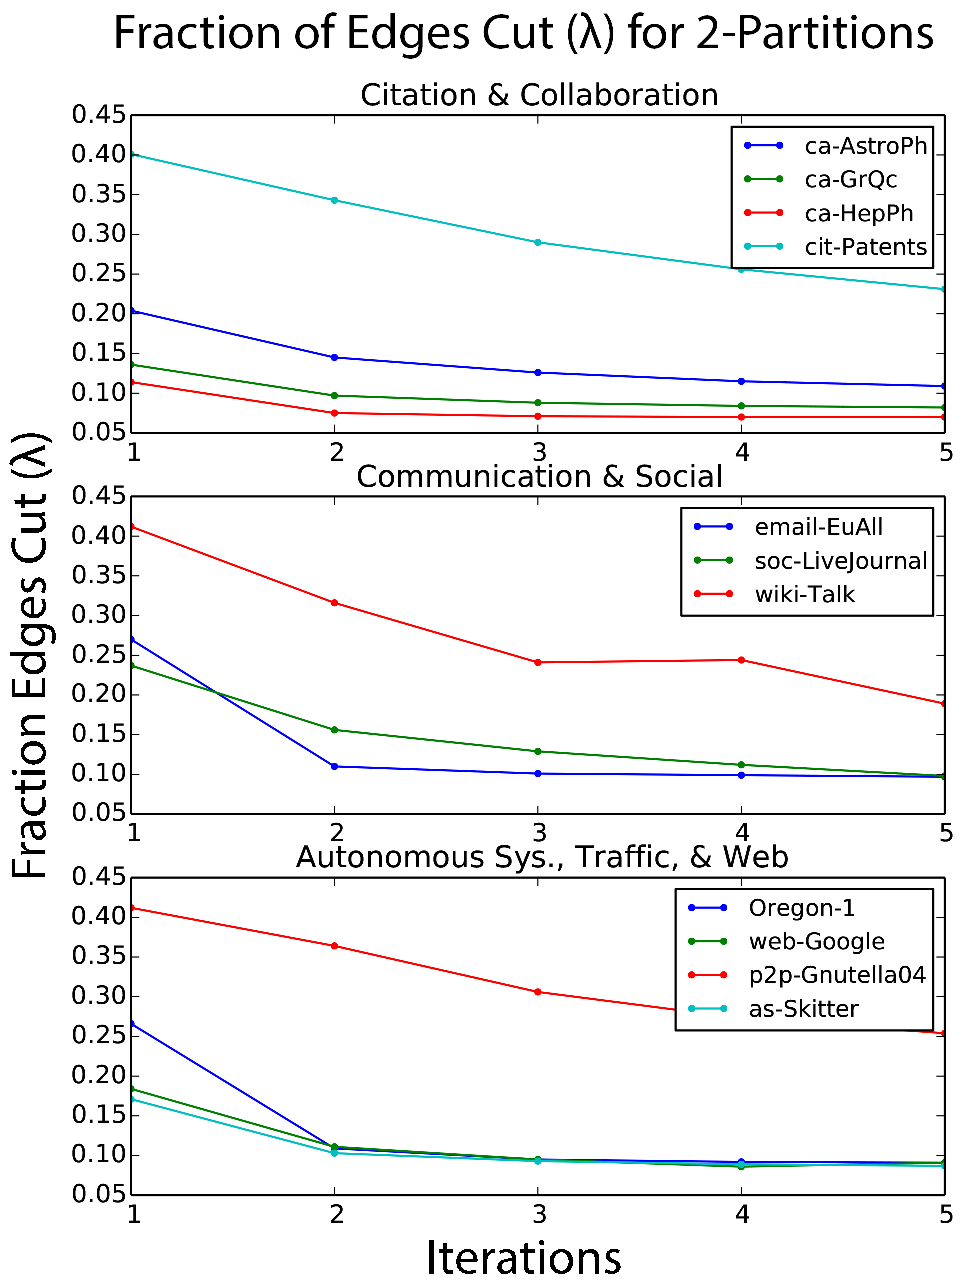
\includegraphics[width=0.9\columnwidth] {figures/real_k2_lambda.pdf}
\caption[Caption for]{Improvement in the edges cut ($\lambda$) over 5 passes for bi-partitions of each graph. Because there are only two partitions, the algorithm is able to quickly fix mistakes it made in the initial partitioning. Many of the errors made in the first pass are fixed in the second iteration, with diminishing improvement thereafter.}
\label{fig:k2_lambda}
\end{figure}

\begin{figure}[t!]
\centering
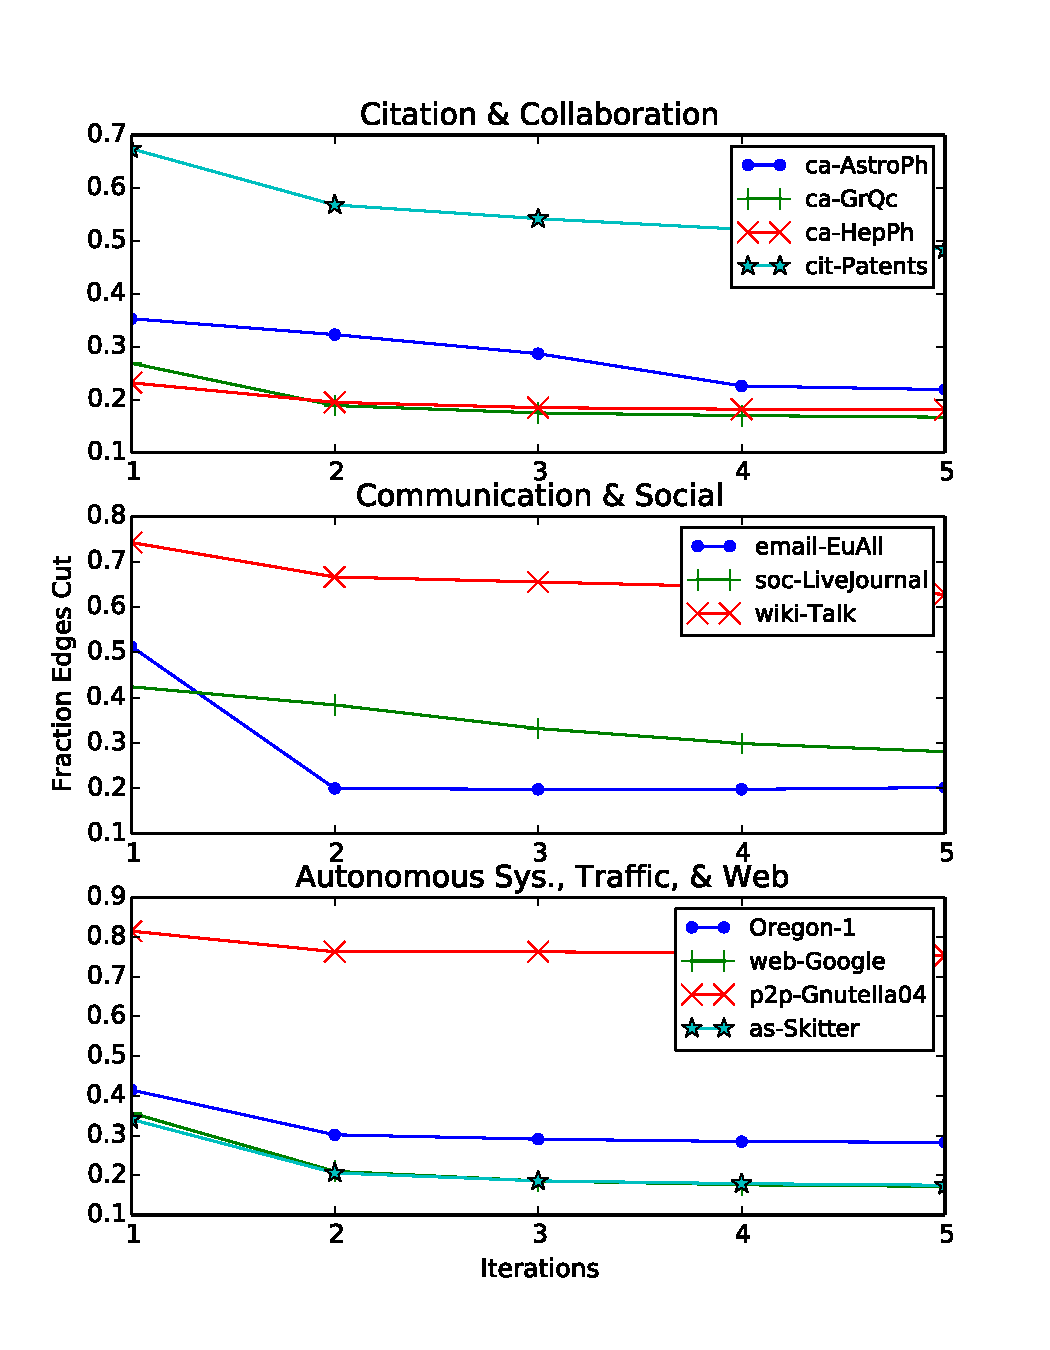
\includegraphics[width=0.9\columnwidth] {figures/real_k16_lambda.pdf}
\caption[Caption for]{Improvement in edges cut ($\lambda$) over 5 passes for $k=16$-partitions of each graph. Dividing the graph into 16 partitions makes the minimum edge cut problem much more challenging. Similar to the bi-partition results, we experience the best gain in the second pass and less in subsequent passes.}
\label{fig:k16_lambda}
\end{figure}


\subsection{Scalability}
In order to test the scalability of \ourmethod we used a series of Kronecker graphs running on a state-of-the-art system.
In Figure~\ref{fig:kronqual} we illustrate the streaming graph partitioner on Kronecker graphs with a widely varying number of nodes.
We show the Kronecker graphs performance in Figure!\ref{fig:kronspeed}. 
\ourmethod is able to achieve a good balance between quality at incredible speeds.


\begin{figure}[h!]
\centering
  
\includegraphics[width=0.8\columnwidth]{figures/kronecker_quality_tests.pdf}
  \caption{Partition quality of various Kronecker graphs.}
  \label{fig:kronqual}
\end{figure}

\begin{figure}[h!]
\centering
  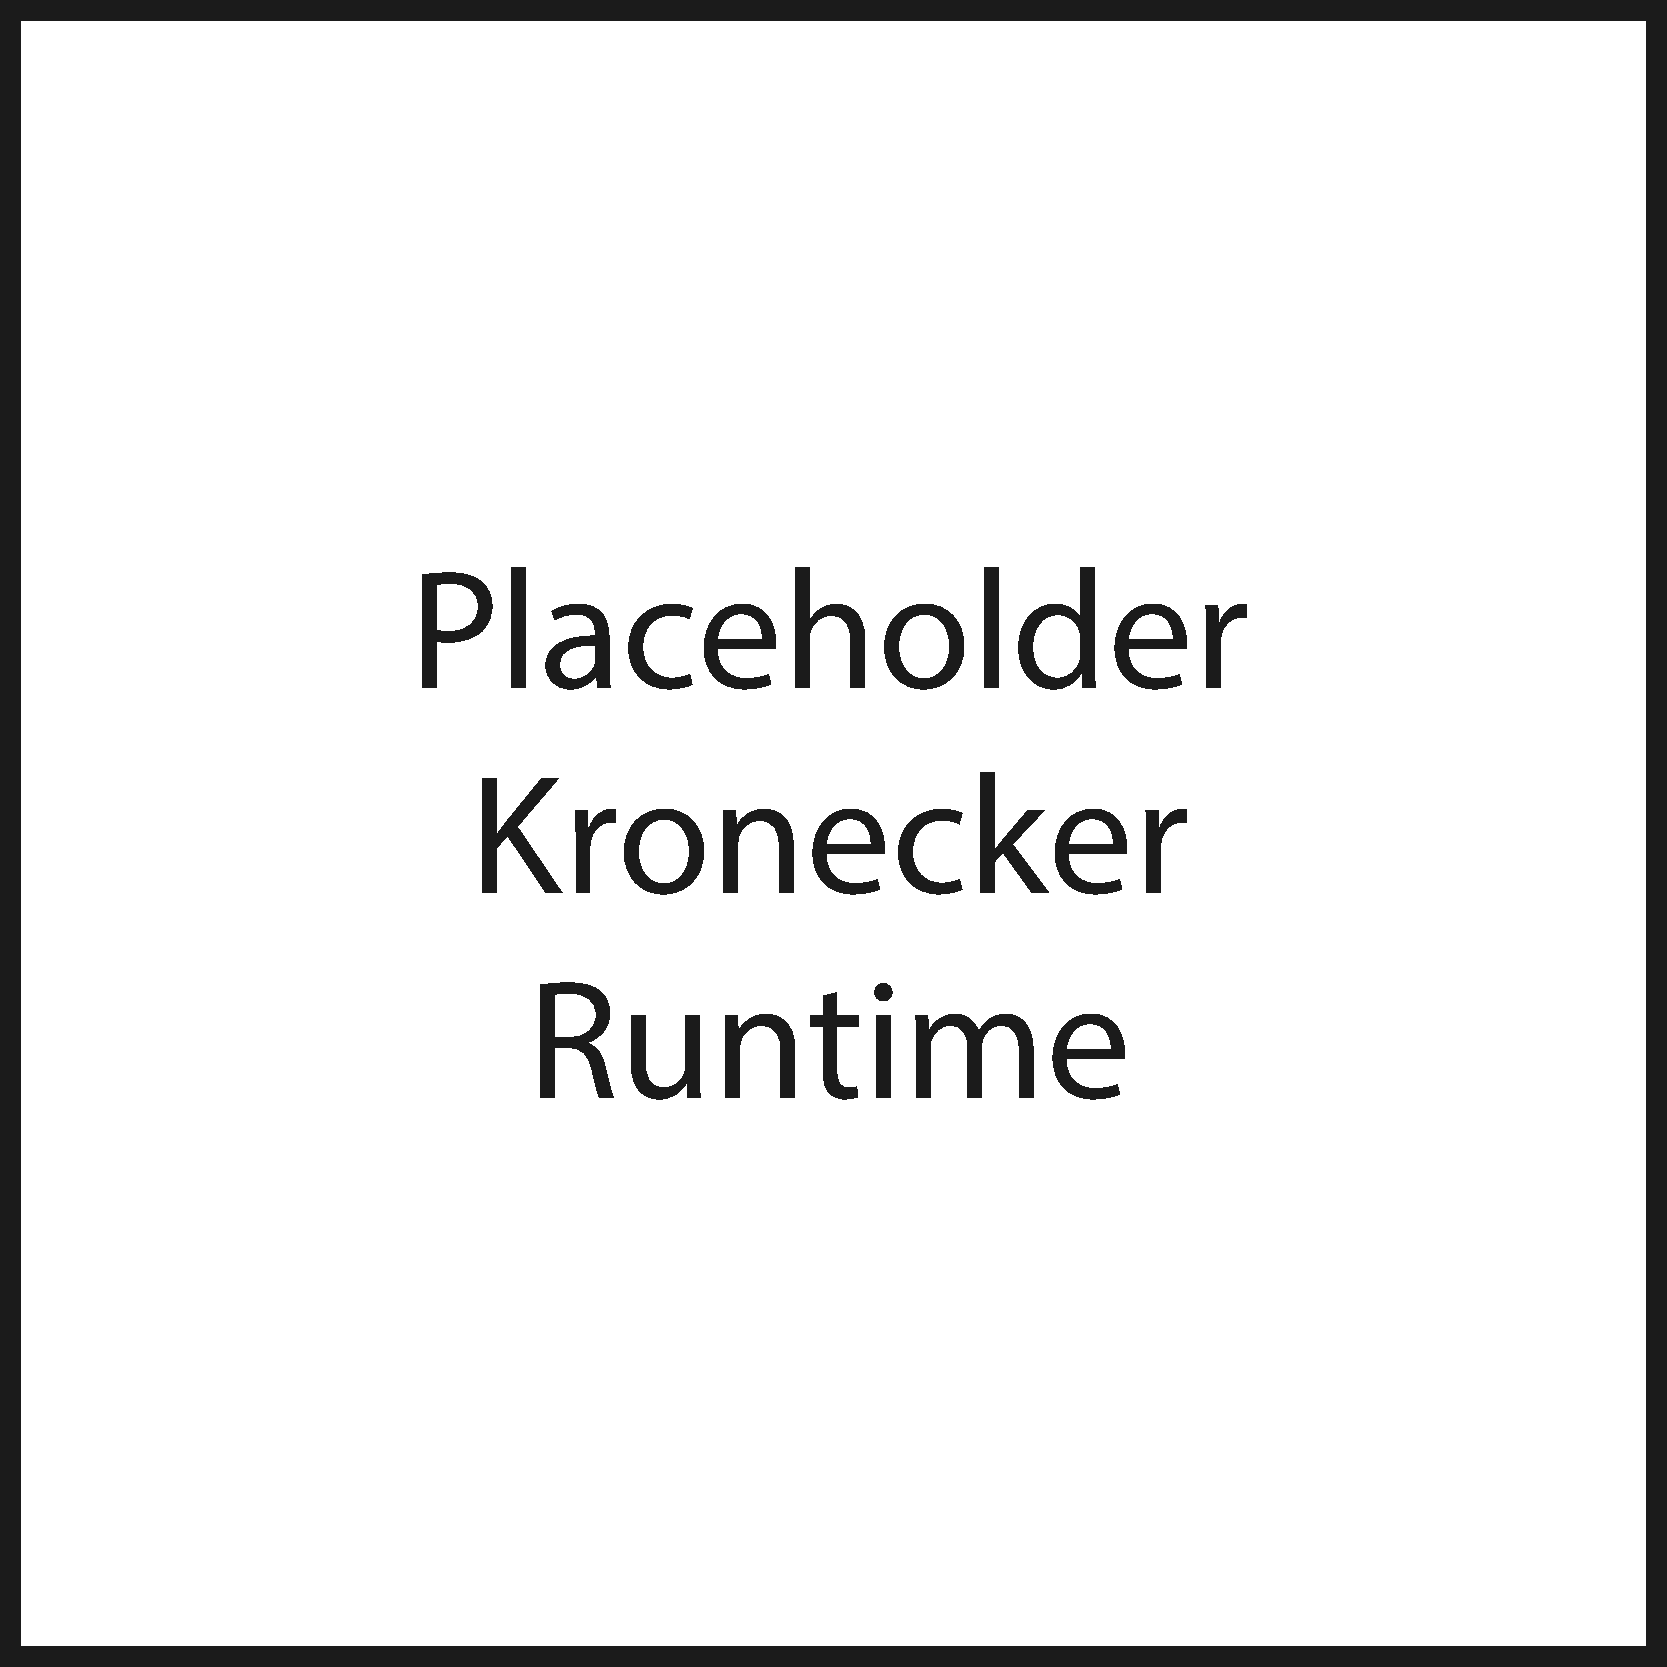
\includegraphics[width=0.8\columnwidth]{figures/kronecker_speed_tests.pdf}
  \caption{Partition speed of various Kronecker graphs.}
  \label{fig:kronspeed}
\end{figure}


\subsection{Analysis}
% Other data from real-world was harder to analyze -- there are not enough wide differences between data sets' results to draw strong conclusions.
Despite the complexity of many of the real graphs, \ourmethod creates well-balanced partitions.
While Power-Law graphs are overwhelmingly considered to be difficult to partition~\cite{Abou-Rjeili:2006:MAP:1898953.1899055}, we have demonstrated that a very simple, fast, algorithm is capable of significantly reducing communication in their parallel computation. 
We also demonstrate in Figures~\ref{fig:k2_lambda, fig:k16_lambda} that additional passes can further reduce edges cut (by up to a factor of 3). 

% Isolated comparisons we have made to the state-of-the-art partitioner METIS show that these results are competitive (usually within a factor of 2).
In Figure~\ref{fig:metis}, \ourmethod performs comparably with parMETIS.  
Streaming partitioning is a valid alternative to conventional offline approaches and can be integrated in distributed-memory, on-the-fly algorithms for big-data.

One set of outlying (poorly-performing) data points are the Gnutella networks.
While Gnutella networks exhibit power-law-like topologies, elements of their algorithm truncate nodes from ever becoming extremely large. 
This heavy-clipping sets the Gnutella networks apart from many of the other social network topologies in our experiments.
The data set also has extremely low clustering coefficients and a very small number of closed triangles \cite{Ripeanu:2002:MGN:613352.613670}. 
Low clustering coefficients decrease the chance that neighbors of the current node-under-consideration share a partition. 
With more neighbors distributed across the partitions, many partitions will have roughly the same score, making optimal partition choices much harder.

A danger of naively running multiple passes is that one partition often becomes populated by very high-degree vertices. 
We attribute this to the ``dense core'' surrounded by a less-dense periphery that many scale-free graphs possess.
This can be observed qualitatively when scale-free graphs are embedded in a spectral space~\cite{Lang04findinggood}.

This dense partition tends to strongly emerge as we continue to make further passes of the streaming algorithm.
In order to overcome this we used the tempered parameter technique described in our methodology section. 


\subsection{Streaming Heuristics}
Given a stream of vertices, a heuristic makes a partition decision, given vertex $v$, and capacity constraint $C$ (where $C$ is generally $\approx \frac{(\epsilon+|V|)}{n}$ Stanton presents the following heuristics, roughly in order from most naive to most complex~\cite{Stanton:2012:SGP:2339530.2339722}: (only the un-buffered heuristics are presented)

\begin{enumerate}
\item \textbf{Balanced:} assign $v$ to partition of minimum size, with random tie breaking.
\item \textbf{Chunking:} divide input stream into chunks of size $C$.
\item \textbf{Hashing:} assign $v$ to $H(v)$, where $H$ is hash function $F:V\to\{1\dots k\}$
\item \textbf{Weighted Deterministic Greedy (WDG):} Assign $v$ to partition that it has most edges to, weighted by the relative size of each partition (weight function can be linear or exponential).
\item \textbf{Weighted Randomized Greedy:} Assign $v$ randomly according to a probability distribution defined by the weights of each partition in WDG.
\item \textbf{Weighted Triangles:} Assign $v$ to partition whose intersection with $v$ contains the most triangles, weighted by the relative size of each partition.
\item \textbf{Balance Big:} for high-degree $v$, use Balanced. For low-degree $v$, use WDG. 
\end{enumerate}

Of note is that many major graph-processing toolkits such as GraphLab~\cite{Low:2012:DGF:2212351.2212354} use the hashed (random) partitioning method, which essentially produces a worst-case edgecut of size $\frac{k-1}{k}|E|$, but which has the benefit that $H(v)$ can be called at any time to return the compute node that owns $v$.


In Stanton's experimental results~\cite{Stanton:2012:SGP:2339530.2339722}, WDG performed far better than any other partitioner.
FENNEL~\cite{tsourakakis2012fennel} is a heuristic that generalizes the WDG partitioner for any weight function, and provides a somewhat more rigorous theoretical framework.
For this project, we always consider a WDG partitioner. 

%!TEX root=kdd15_workshop_main.tex
\section{Conclusion} \label{sec:conc}
In this work, we demonstrated \ourmethod, a \emph{distributed, streaming} partitioner. 

While Power-Law graphs are considered to be very difficult to partition~\cite{Abou-Rjeili:2006:MAP:1898953.1899055}, we have demonstrated that a very simple, fast algorithm is capable of significantly reducing communication in their parallel computation. Using the methodology outlined by Nishimura and Ugander~\cite{nishimura2013restream} and applying an HPC framework we have scaled the partitioning process to graphs with billions of nodes in a matter of seconds, while more sophisticated graph partitioners struggle on graphs that are orders of magnitude smaller.

We have demonstrated our implementation on both real world and high-scale synthetic graphs on a leading supercomputer. \ourmethod is scalable and can partition a graph of \largestgraphedges edges in \largestgraphtime, while maintaining partition quality comparable to what competing implementations achieve on smaller-scale graphs. 


%\subsection{References}
\bibliographystyle{abbrv}
\bibliography{bibly}
% \thebibliography
%\balancecolumns % GM June 2007
\end{document}

